\section{Composition Filters in \Compose*{}}
\label{sec:CompositionFiltersInComposeStar}
A \Compose* application consists of concerns that can be divided in three parts: filter module specification, superimposition, and implementation. A filter module contains the filter logic to filter on messages that are incoming or outgoing the superimposed object. A message has a target, which is an object reference, and a selector, which is a method name. The superimposition part specifies which filter modules, annotations, conditions, and methods need to be superimposed on which objects. The implementation part contains the class implementation of the concern. How these parts are placed in
a concern is shown in \autoref{lst:concerntemplate}.

\begin{lstlisting}[language={Composestar},style=floatlisting,%
                   caption={Abstract concern template},label={lst:concerntemplate},%
                   floatplacement=hbp]%removed "t" so that it is not longer breaking the history list
concern{
  filtermodule{
    internals
    externals
    conditions
    inputfilters
    outputfilters
  }
  
  superimposition{
    selectors
    filtermodules
    annotations
    constraints
  }
  
  implementation
}
\end{lstlisting}

\begin{figure}
  \centering
  \includegraphics[style=thirdheight]{cfmodel}
  \caption{Components of the composition filters model}
  \label{fig:cfmodel}
\end{figure}
The working of the filter module is shown in \autoref{fig:cfmodel}.
A filter module can contain input and output filters. The difference between these two
sets of filters is that the first is used to filter on incoming messages and the second 
filter set is used on the outgoing messages. A return of a method is not considered as an outgoing message.
A filter has three parts: the filter identifier, 
the filter type, and one or more filter elements. The filter element exist out of an optional condition part, a matching part, and a substitution part. These parts are shown below:

\begin{center}
$\overbrace{stalker\_filter}^{identifier}:\overbrace{Dispatch}^{filter~type}~=~\{\overbrace{!pacmanIsEvil}^{condition~part}
=>\overbrace{[*.getNextMove]}^{matching~part}~\overbrace{stalk\_strategy.getNextMove}^{substitution~part}~\}$
\end{center}

The filter identifier is the unique name for a filter in a filter module. 
A filter matches when both the condition as the matching provide the boolean value true.
In the demonstrated filter it matches on every
message where the selector is \lstinline!getNextMove!, the `*' in the target means that every target matches.
When the condition part and the matching part are true, the message is substituted with the values of the substitution part. How these values are substituted and
how the message continues depends on the filter type. At the moment there are four basic filter types in \Compose*; it is possible to write custom filter types.

\begin{description}[style=nextline,noitemsep]
\item [Dispatch] If the message is accepted, it is dispatched to the specified target of the message,
otherwise the message continues to the subsequent filter. This filter type can only be used for
input filters;
\item [Send] If the message is accepted, it is sent to the specified target of the message,
otherwise the message continues to the subsequent filter. This filter type can only be used for
output filters;
\item [Error] If the filter rejects the message, it raises an exception, otherwise the message continues
to the next filter in the set;
\item [Meta] If the message is accepted, the message is sent as a parameter of another meta message
to an internal or external object, otherwise the message just continues to the next filter. The object that receives the
meta message can observe and manipulate the message and can re-activate the execution of the message.
\end{description}

The \lstinline|pacmanIsEvil| used in the condition part must be declared in the conditions section of
a filtermodule. The targets that are used in a filter must declared as internals or externals.
Internals are objects which are unique for each instance of a filter module and
externals are shared between filter modules.

The filter modules can be superimposed on classes with filter module binding, this binding
has a selection of objects on one side and a filter module on the other side. The selection
is defined with a selector definition. The selector uses predicates, such as
\lstinline|isClassWithNameInList|, \lstinline|isNamespaceWithName|, and \lstinline|namespaceHasClass|,
to select objects. It is also possible to bind conditions, methods, and annotations to classes with the use of superimposition.

The last part of the concern is the implementation part. In the implementation part we can define the object behavior of the concern, so for example in a logging concern, we can define specific log functions.
